\chapter{Modelos booleanos basados en objetos estoc\'asticos}
\label{ch3:booleanModels}

La presente revisi\'on se basa principalmente en el libro de \citet{lantuejoul_geostatistical_2002} pero se explican algunos conceptos mas detalladamente.

Los modelos booleanos, aunque simples en la idea intuitiva detr\'as de las matem\'aticas requieren otros ingredientes a\'un m\'as esenciales.
En particular, primero se presenta una breve rese\~na de la teor\'ia de procesos puntuales. Posteriormente se definen los modelos booleanos. Para la simulacion de dichos modelos son necesarios las bases te\'oricas presentadas en las dos secciones antes de la secci\'on de simulaci\'on y en la \'ultima secci\'on se presenta un caso teoricamente importante.

\section{Procesos puntuales}

Un proceso puntual aleatorio es un modelo estoc\'astico \citep{lantuejoul_geostatistical_2002} en el cual cada realizaci\'on est\'a formada por un n\'umero finito o contable de puntos en $\mathbb{R}^d$.

Aunque los elementos de un proceso puntual son muy b\'asicos, estos procesos pueden formar estructuras complicadas. La \autoref{f:pointProc} muestra algunos ejemplos, pero existe una gran variedad de modelos. Adem\'as, en muchos fen\'omenos la simplificaci\'on de eventos espaciales a puntos es bastante adecuada. Por ejemplo, para modelar \'arboles en los bosques, epicentros de terremotos, estrellas en las galaxias, entre otros. Una raz\'on m\'as de la importancia de los procesos puntuales, es que ellos sirven de ingredientes para modelos m\'as complicados como en los que se enfoca esta tesis.

\DTLloaddb[noheader=false]{ppHom}{code/datasets/ppHom.csv}
\DTLloaddb[noheader=false]{ppInHom}{code/datasets/ppInHom.csv}
\DTLloaddb[noheader=false]{ppCluster}{code/datasets/ppCluster.csv}
\begin{figure}
	\centering
\begin{tikzpicture}[scale=4.5]
        \draw[color=lightgray, thick, fill=white] (-0.03,-0.03) rectangle (1.03,1.03);
	\DTLforeach*{ppHom}{\x=x, \y=y}{\path[fill=blue] (\x,\y) circle (0.015);}
\end{tikzpicture}
\hfill
\begin{tikzpicture}[scale=4.5]
        \draw[color=lightgray, thick, fill=white] (-0.03,-0.03) rectangle (1.03,1.03);
	\DTLforeach*{ppInHom}{\x=x, \y=y}{\path[fill=blue] (\x,\y) circle (0.015);}
\end{tikzpicture}
\hfill
\begin{tikzpicture}[scale=4.5]
        \draw[color=lightgray, thick, fill=white] (-0.03,-0.03) rectangle (1.03,1.03);
	\DTLforeach*{ppCluster}{\x=x, \y=y}{\path[fill=blue] (\x,\y) circle (0.015);}
\end{tikzpicture}
	\caption{Ejemplos de procesos puntuales. a) Caso Homog\'eneo, b) Intensidad no uniforme c) Proceso de conglomerados.}
%\protect\hypertarget{_Ref405932721}{}{}Figura 13. 
	\label{f:pointProc}
\end{figure}

%\begin{figure}[H]
    %\centering
    %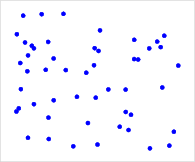
\includegraphics{pointProcessHom} \hfill
    %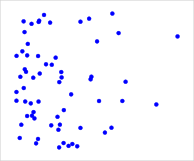
\includegraphics{pointProcessInhom} \hfill
    %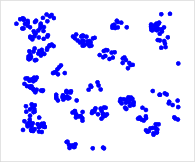
\includegraphics{pointProcessCluster}
    %\caption{Name}
    %\label{fig:pointProcPGF}
%\end{figure}


En un proceso puntual \textit{localmente finito} el n\'umero de puntos dentro de cualquier conjunto compacto (cerrado y acotado) es casi seguramente finito.
En este caso es conveniente describir las propiedades estad\'isticas del proceso puntual mediante un conteo del n\'umero de puntos dentro de subconjuntos del espacio.
Sea $N(B)$ el n\'umero aleatorio de puntos dentro del conjunto $B$, denominado el funcional que cuenta. $B$ es un elemento de $\mathcal{B}_0$, el conjunto de los Borelianos acotados.

La distribuci\'on espacial de un \textbf{proceso homog\'eneo de Poisson} con intensidad $\theta$ est\'a caracterizado por las siguientes propiedades:

\begin{enumerate}
	\item Si $A \in \mathcal{B}_0$, entonces el n\'umero de puntos dentro de $A$, $N(A)$, es una variable aleatoria de Poisson con par\'ametro $\lambda \|A\|$ donde $\|A\|$ es el $d$-volumen de $A$
		\begin{equation*}
			P\{N(A) = n\} =
			exp\{-\lambda \|A\|\}
			\frac{[\lambda \|A\|]^n}{n!}
		\end{equation*}
	\item Si $(A_i, i \in I)$ es una familia finita de elementos disjuntos de $\mathcal{B}_0$, entonces las variables aleatorias $N(A_i), i \in I)$ son mutuamente independientes.
\end{enumerate}

Dado que el valor medio de la distribuci\'on de Poisson es igual a su par\'ametro $\lambda$, la media del n\'umero de puntos sobre $A$ es igual a $\lambda \|A\|$. En particular, $\lambda$ es la media del n\'umero de puntos por unidad de $d$-volumen. Si se requiere simular una cantidad exacta de puntos, entonces $\|A\| / n = <~\lambda~>$ da un valor (medio $<\cdot>$) aproximado de la intensidad. Sin embargo, esta intensidad calculada no es la \'unica porque existe un conjunto no-numerable de valores de intensidad que pueden producir el mismo $n$.

El siguiente teorema, cuya demostraci\'on se puede encontrar en \cite[p. 121]{lantuejoul_geostatistical_2002}, muestra que los puntos de un proceso puntual homog\'eneo de Poisson son independientes y con ubicaci\'on totalmente aleatoria.

Sea $A \in \mathcal{B}_0$. Si $N(A)=n$, los $n$ puntos son independientes y uniformemente distribuidos en $A$.

Este teorema permite un algoritmo simple para simular un proceso puntual de Poisson en una regi\'on A.

\begin{enumerate}
	\item Inicialice el conjunto $X = \emptyset$,
	\item Obtenga cu\'antos puntos van a ser simulados al muestrear $n \sim Poisson(\theta \|A\|)$,
	\item si $n > 0$, para $i=1, \ldots,n$ genere $x_i \sim Unif(A)$,
	\item Los puntos $x_i \in \mathbb{R}^d$ pertenecientes a la realizaci\'on del proceso puntual son $X=\{x_1, \dots, x_n\}$.
\end{enumerate}

Computacionalmente, $X$ puede ser un arreglo bidimensional de $n \times d$, $n$ renglones por $d$ columnas. Aunque este algoritmo es computacionalmente r\'apido, se puede hacer m\'as eficiente si se toma en cuenta el orden de este arreglo ($n \times d$ \'o $d \times n$); dependiendo del paradigma en la memoria: row-major vs column-major \citep{karniadakis_parallel_2003,matloff_parallel_2016}.

El lenguaje de programaci\'on utilizado para desarrollar esta tesis fue \verb|R| ya que fue dise\~nado para desarrollos estad\'isticos y hay varios paquetes ya disponibles en su repositorio que complementan a este trabajo. A lo largo de esta tesis se referir\'a una funci\'on de alg\'un paquete de \verb|R| escribi\'endola con la siguiente sintaxis \verb|paquete::funcion|.

El algoritmo para generar realizaciones de un proceso puntual de Poisson est\'a computacionalmente implementado en la funci\'on \verb|spatstat::rpoint| del software \verb|R|. Si ya se sabe el valor de $n$, entonces la funci\'on que simula los puntos, dentro del mismo software, se llama \verb|spatstat::runifpoint|.

Los mejores ejemplos para la metodolog\'ia mostrada en esta tesis se obtuvieron con procesos puntuales homog\'eneos en los cuales $\lambda$ es constante. Otros modelos comunes son cuando $\lambda$ var\'ia espacialmente (Proceso puntual de Poisson no homog\'eneo) y cuando la intensidad espacial es una funci\'on aleatoria (Proceso de Cox).

\section{Construcci\'on del modelo booleano}

Se necesitan dos ingredientes b\'asicos e independientes para la construcci\'on de un modelo booleano en $\mathbb{R}^d$:

\begin{enumerate}
\item Un conjunto de \textit{semillas}, esto es, un proceso puntual de Poisson $\mathcal{P}$ con funci\'on de intensidad $\theta=(\theta(x),\ x\in\mathbb{R}^d)$.
    \item Una familia $(A(x),x\in\mathbb{R}^d)$ de subconjuntos de $\mathbb{R}^d$ compactos, no vac\'ios, aleatorios e independientes. Al subconjunto $A(x)$ se le llama el \textit{objeto implantado en} $x$ y su funcional que pega se denota por $\mathcal{T}_x$.
\end{enumerate}

De este modo, un modelo booleano $X$ es la \textit{uni\'on de todos los objetos implantados en las semillas Poisson}

\[X=\bigcup_{x\in\mathcal{P}}A(x)\]

La apariencia de una realizaci\'on del modelo depende en gran medida de la forma que tengan los objetos. \'Estos pueden ser, por ejemplo, segmentos de recta, discos, pol\'igonos, etc\'etera. En la \autoref{f:boolEx} se muestran dos realizaciones de modelos booleanos. En el primer caso se muestra un conjunto de c\'irculos --los objetos-- implantados sobre semillas de Poisson homog\'eneamente distribuidas. Y en el segundo caso se muestra otra realizaci\'on en el cual los objetos son segmentos rectil\'ineos.

\begin{figure}[H]
	\centering
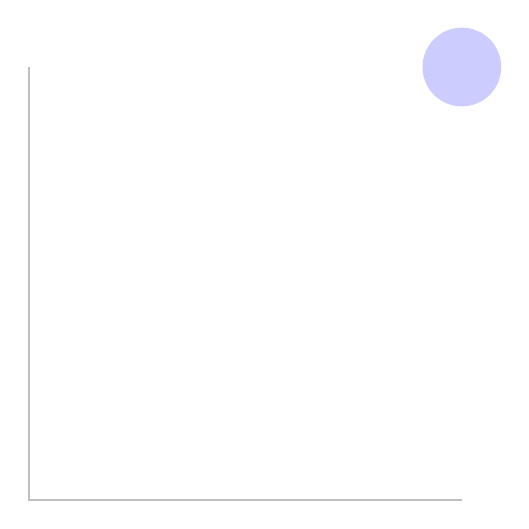
\begin{tikzpicture}[scale=5]
	\draw[lightgray, thick] (-0.1,1) -- (-0.1,-0.1) -- (1,-0.1);
\DTLforeach*{ppHom}{\x=x, \y=y}{\path [fill=blue, fill opacity=0.2] (\x,\y) circle (0.1cm);}
\end{tikzpicture}
%\hfill
%\begin{pgfpicture}% example from tikz manual 3.0.1
	%\pgfmathdeclarerandomlist{color}{{red}{blue}{green}{yellow}{white}}
	%\foreach \a in {1,...,50}{
		%\pgfmathrandominteger{\x}{1}{85}
		%\pgfmathrandominteger{\y}{1}{85}
		%\pgfmathrandominteger{\r}{5}{10}
		%\pgfmathrandomitem{\c}{color}
		%\pgfpathcircle{\pgfpoint{+\x pt}{+\y pt}}{+\r pt}
		%\color{\c!40!white}
		%\pgfsetstrokecolor{\c!80!black}
		%\pgfusepath{stroke, fill}
	%}
%\end{pgfpicture}
\qquad
\qquad
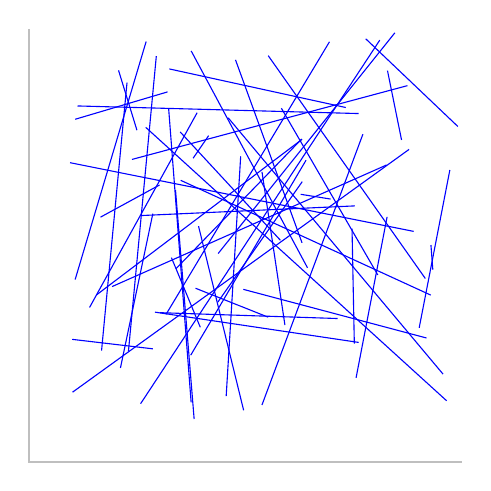
\begin{tikzpicture}[scale=5]
	\draw[lightgray, thick] (-0.1,1) -- (-0.1,-0.1) -- (1,-0.1);
	%\draw[lightgray, thick] (0,1) -- (0,0) -- (1,0);
	\foreach \x in {1,2,...,50}{
	\draw[blue] (rnd,rnd) -- (rnd,rnd);}
\end{tikzpicture}
\caption{Ejemplos de modelos booleanos cuyos objetos son (a) c\'irculos;
%b) modelo booleano con m\'as atributos denotdaos por el color y el tama\~no de  los objetos circulares;
b) Segmentos lineales.}
\label{f:boolEx}
\end{figure}

Ya que un modelo booleano es posiblemente la uni\'on de una infinidad de objetos, no existe garant\'ia de que sea cerrado. Este ser\'a ciertamente el caso si para cada punto $x\in\mathbb{R}^d$ existe una vecindad a la cual s\'olo le pega una cantidad finita de objetos (casi seguramente), y en particular si la poblaci\'on de objetos $(A(x),x\in\mathcal{P})$ es de orden finito. Espec\'ificamente, sea $N(K)$ el n\'umero de objetos que le pegan al compacto $K$. Entonces

\[N(K)=\sum_{x\in\mathcal{P}}\mathbbm{1}_{K\cap A(x)\neq\emptyset}.\]

Un c\'alculo sencillo muestra que la media de $N(K)$ es

\[\vartheta(K)=\int_{\mathbb{R}^d}\theta(x)\mathcal{T}_x(K)dx\ \leq\ \infty.\]

Se dice que un modelo booleano es de \textbf{orden finito} si $\vartheta(K)<\infty\ \forall\ K\in\mathcal{K}$. A lo largo de este texto se supondr\'a que los modelos booleanos considerados son de orden finito.

\section{El funcional que evita (avoiding functional) del modelo booleano}

Comencemos determinando la distribuci\'on del n\'umero de objetos que intersectan al subconjunto compacto $K$.

Se tendr\'a que $N(K)$ es una variable aleatoria Poisson con media $\vartheta(K)$: Para cada $D\in\mathcal(K)$ consideremos el n\'umero $N_D(K)$ de objetos implantados en $D$ que le pegan a $K$.

\[N_D(K)=\sum_{x\in\mathcal{P}\cap D}\mathbbm{1}_{K\cap A(x)\neq\emptyset}.\]

Por definici\'on, el n\'umero de puntos en $\mathcal{P}\cap D$ sigue una distribuci\'on Poisson con media

\[\theta(D)=\int_D \theta(x)dx.\]

Supongamos que este n\'umero es igual a $n$. De acuerdo a las propiedades de un proceso puntual de Poisson estos puntos est\'an distribuidos de manera uniforme e independiente sobre $D$, con funci\'on de densidad de probabilidad $\frac{\theta(\cdot)}{\theta(D)}$. M\'as a\'un, un objeto implantado en $x$ le pega a $D$ con probabilidad $\mathcal{T}_x(K)$ y lo evita con la probabilidad complementaria $1-\mathcal{T}_x(K)$. En consecuencia, la funci\'on generadora de $N_D(K)$ es

\[\mathbb{E}\left\{s^{N_D(K)}\right\}=\sum_{n=0}^\infty e^{-\theta(D)}\frac{\theta(D)^n}{n!}\left(\int_D\frac{\theta(x)}{\theta(D)}[(1+(s-1)\mathcal{T}_x(K)]dx\right)^n,\]

donde $0\leq s\leq 1$, y al sumar se tiene que

\[\mathbb{E}\left\{s^{N_D(K)}\right\}=\exp\left\{(s-1)\int_D\theta(x)\mathcal{T}_x(K)dx\right\}.\]

Para extender este resultado a todo el espacio, sea $(D_n,n\in\mathbb{N})$ una sucesi\'on creciente de compactos que cubren a $\mathbb{R}^d$. Entonces $(N_{D_n}(K),n\in\mathbb{N})$ tambi\'en es una sucesi\'on creciente y converge casi seguramente a $N(K)$. En consecuencia

\[\mathbb{E}\left\{s^{N(K)}\right\}=\lim_{n\rightarrow\infty}\mathbb{E}\left\{s^{N_{D_n}(K)}\right\}=exp\left\{(s-1)\int_{\mathbb{R}^d}\theta(x)\mathcal{T}_x(K)dx\right\}.\]

Esta \'ultima expresi\'on se reconoce como la funci\'on generadora de una distribuci\'on Poisson con media $\vartheta(K)$.

Ya que $\mathbb{P}\{X\cap K=\emptyset\}=\mathbb{P}\{N(K)=0\}$, deducimos que el funcional que evita del modelo booleano es

\[\mathbb{P}\{X\cap K=\emptyset\}=e^{-\vartheta(K)},\ \ K\in\mathcal{K}.\]

\section{Propiedades de estabilidad}

Para poder explorar las propiedades de estabilidad del modelo booleano es necesario echar mano de conceptos b\'asicos de morfolog\'ia, a saber, el concepto de \textit{dilataci\'on}.

 Dados $x\in\mathbb{R}^d$ y $A\subset\mathbb{R}^d$, $A_x$ denota al conjunto obtenido al trasladar $A$ por $x$. Si $B$ es un subconjunto de $\mathbb{R}^d$ entonces la \textit{suma de Minkowski} de $A$ y $B$ es

\[A\oplus B = \bigcup_{y\in B}A_y.\]

Decimos entonces que el punto $x$ pertenece al conjunto $A$ \textit{dilatado} por $B$ si $B_x$ le pega a $A$ (es decir, si $B_x\cap A\neq\emptyset$.

Por otra parte, necesitaremos tambi\'en el concepto de $i$-planos, los cuales son espacios afines de dimensi\'on $i$. [Un espacio af\'in es un espacio vectorial sin origen].

Las propiedades b\'asicas de estabilidad de un modelo booleano son:

\begin{itemize}
	\item La uni\'on de dos modelos booleanos independientes es un modelo booleano.
	\item Un modelo booleano dilatado por un subconjunto compacto no vac\'io de $\mathbb{R}^d$ es un modelo booleano.
	\item La intersecci\'on de un modelo booleano con un subconjunto compacto de $\mathbb{R}^d$ es un modelo booleano.
	\item La intersecci\'on de un modelo booleano y un $i$-plano es un modelo booleano.
\end{itemize}

A continuaci\'on, se proporcionan argumentos para justificar estas afirmaciones:

Sean $X'$ y $X''$ dos modelos booleanos independientes con funciones de identidad $\theta'$ y $\theta''$, y funcionales que pegan $\mathcal{T}'$ y $\mathcal{T}''$. Debido a la independencia se tiene que

\[\begin{array}{ccl}
\mathbb{P}\{(X'\cup X'')\cap K=\emptyset\}&=&\mathbb{P}\{X'\cap K=\emptyset\}\mathbb{P}\{X''\cap K=\emptyset\}\\
&&\\
&=&\exp\left\{-\int_{\mathbb{R}^d}\theta'(x)\mathcal{T}'_x(K)+\theta''(x)\mathcal{T}_x''(K)dx\right\}\\
&&\\
&=&\exp\left\{-\int_{\mathbb{R} ^d}\theta(x)\mathcal{T}_x(K)dx\right\}
\end{array}\]

donde $\theta=\theta'+\theta''$ y $\mathcal{T}_x$ queda definido como

\[\mathcal{T}_x(K)=\frac{\theta'(x)}{\theta'(x)+\theta''(x)}\mathcal{T}'_x(K)+\frac{\theta''(x)}{\theta'(x)+\theta''(x)}\mathcal{T}''_x(K),\ \ K\in\mathcal{K}.\]

Este es el funcional que pega de un objeto aleatorio igual a $A'(x)$ con probabilidad $\frac{\theta'(x)}{\theta'(x)+\theta''(x)}$, e igual a $A''(x)$ con probabilidad complementaria $\frac{\theta''(x)}{\theta'(x)+\theta''(x)}$. Este hecho prueba la primera propiedad.

Ahora bien, sea $D$ un subconjunto de $\mathbb{R}$ compacto y no vac\'io. La segunda propiedad es consecuencia directa de la distributividad de la suma de Minkowski sobre la uni\'on de conjuntos:

\[X\oplus D=\bigcup_{x\in\mathcal{P}}A(x)\oplus D.\]

De este modo, la dilataci\'on de un modelo booleano vuelve a ser la uni\'on de objetos aleatorios implantados en las semillas determinadas por $\mathcal{P}$, lo cual determina un nuevo modelo booleano. La diferencia es que en lugar de tener los objetos aleatorios originales $A(x)$, se tienen los objetos aleatorios dilatados $A(x)\oplus D$.

En cuanto a la tercera propiedad, podemos escribir simplemente $X\cap D=\bigcup_{x\in\mathcal{P}}A(x)\cap D$. Sin embargo, esta f\'ormula es dif\'icil de interpretar ya que los objetos $A(x)\cap D$ ser\'an casi seguramente vac\'ios. En cambio, consideraremos la siguiente expresi\'on:

\[\begin{array}{ccl}
\mathbb{P}\{(X\cap D)\cap K=\emptyset\}&=&\mathbb{P}\{X\cap (D\cap K)=\emptyset\}\\
&&\\
&=&\exp\left\{-\int_\mathbb{R}^d\theta(x)\mathcal{T}_x(D\cap K)dx\right\}\\
&&\\
&=&\exp\left\{-\int_\mathbb{R}^d\mathcal{T}_x(D)\frac{\theta(x)\mathcal{T}_x(D\cap K)}{\mathcal{T}_x(D)}dx\right\}
\end{array}
.\]

Pero $\frac{\theta(x)\mathcal{T}_x(D\cap K)}{\mathcal{T}_x(D)}$ es el funcional que pega de $A(x)\cap D$, ya que este objeto es no vac\'io. En consecuencia, $X\cap D$ es un modelo booleano con funci\'on de intensidad $\theta\mathcal{T}(D)$ y funcional que pega $\frac{\theta\mathcal{T}(D\cap K)}{\mathcal{T}(D)}$.

Finalmente, sea $P$ un $i$-plano de $\mathbb{R}^d$. La \'ultima propiedad se puede deducir de la tercera tomando una sucesi\'on creciente de compactos no vac\'ios $(D_n,n\in\mathbb{N})$ que converja a $P$.

El modelo booleano es un caso especial de los modelos basados en objetos. Una primera extensi\'on consiste en reemplazar el proceso puntual de Poisson que especifica la localizaci\'on de los objetos a trav\'es de un proceso espacial de nacimiento y muerte (Preston, 1977; Stoyan et al., 1987). Tambi\'en es posible permitir dependencia entre los objetos. En ese caso, un objeto se inserta o se elimina dependiendo de una funci\'on de los objetos ya presentes (y no solamente el n\'umero de \'estos). Esto lleva al concepto de un proceso de vida y muerte de objetos en el espacio. Un ejemplo t\'ipico es el modelo de interacci\'on dos a dos considerado por Sylverseen y Omre (1994). La primera versi\'on de este modelo incluy\'o un n\'umero fijo de objetos, lo cual permit\'ia la simulaci\'on a trav\'es de un muestreo de Gibbs. Esta restricci\'on fue eliminada en un art\'iculo posterior (1997). Es posible extender el modelo de muchas otras maneras, como el proceso de saltos de Markov de objetos.


\section{Simulaci\'on del modelo booleano}

El problema entre manos es simular el modelo booleano en $D$, sujeto a las condiciones de que dos subconjuntos finitos $C_0$ y $C_1$ deben estar contenidos en $X^c$ y $X$, respectivamente. Este problema es importante en la industria petrolera. Los ingenieros petroleros requieren conocer la geometr\'ia del yacimiento para poder ejecutar programas de simulaci\'on de flujos. Un algoritmo desarrollado por Haldersen en 1983 fue notablemente mejorado por Chessa en 1995. Consiste en simular de manera independiente los cuerpos arenosos (los objetos) que intersecan los pozos y aquellos que no. Esta perspectiva dicot\'omica es posible gracias a las propiedades de independencia del proceso Poisson. La dificultad de esta estrategia es que la distribuci\'on de un objeto que interseca al pozo depende no solamente de d\'onde est\'e implantado, sino tambi\'en del n\'umero y la localizaci\'on de los pozos que interseca. Usualmente, el problema se vuelve intratable en cuanto este n\'umero es mayor a uno.

El algoritmo iterativo descrito a continuaci\'on fue dise\~nado a partir de comunicaciones privadas entre Matheron y Lantu\'ejoul en 1990. Posteriormente Gedler (1991) llevo a cabo el trabajo preliminar bajo la supervisi\'on de Lantu\'ejoul. Ya que este algoritmo de simulaci\'on condicional es una versi\'on modificada de un algoritmo de simulaci\'on no condicional (mediante la restricci\'on del kernel de transici\'on), se presenta primero el algoritmo de simulaci\'on no condicional.

Se discuti\'o anteriormente que $X\cap D$ es un modelo booleano con funci\'on de intensidad $\theta(\cdot)\mathcal{T}_x(D)$. De manera acorde, el n\'umero de objetos de $X\cap D$ es de distribuci\'on Poisson con media

\[\vartheta(D)=\int_{\mathbb{R}^d}\theta(x)\mathcal{T}_x(D)dx.\]

El funcional que pega de un objeto de $X\cap D$ implantado en $x$ es $\frac{\mathcal{T}_x(D\cap\cdot)}{\mathcal{T}_x}(D)$.

Un \textit{objeto t\'ipico} de $X\cap D$ es un objeto seleccionado uniformemente entre los objetos de $X\cap D$. Un objeto t\'ipico de $X\cap D$ se implanta de acuerdo a la funci\'on de densidad $\theta(\cdot)\mathcal{T}(D)$.  Su funcional que pega es

\[\mathcal{T}(K)=\int_{\mathbb{R}^d}\frac{\theta(x)\mathcal{T}_x(D)}{\vartheta(D)}\frac{\mathcal{T}_x(D\cap K)}{\mathcal{T}_x(D)}=\frac{1}{\vartheta(D)}\int_{\mathbb{R}^d}\theta(x)\mathcal{T}_x(D\cap K)dx\]
\vspace{0.1in}
Notemos que en particular $\mathcal{T}(D)=1$ y $\mathcal{T}(K)=0$ si $K$ es disjunto de $D$.

Por otra parte, $X\cap D$ tiene la misma distribuci\'on que una uni\'on de $N$ objetos t\'ipicos independientes, donde $N$ tiene distribuci\'on Poisson con media $\vartheta(D)$. Este hecho se prueba del siguiente modo: Sea $Y$ tal uni\'on. Su funcional que evita es

\[\begin{array}{ccl}\mathbb{P}\{Y\cap K=\emptyset\}&=&\sum_{n=0}^\infty e^{-\vartheta(D)}\frac{\vartheta(D)^n}{n!}[1-\mathcal{T}(K)]^n\\
&&\\
&=&exp\{-\vartheta(D)\mathcal{T}(K)\}\\
&&\\
&=&exp\left\{-\int_{\mathbb{R}^d}\theta(x)\mathcal{T}_x(D\cap K)dx\right\}
\end{array}\]

el cual resulta ser exactamente el funcional que evita de $X\cap D$.

En consecuencia, una simulaci\'on no condicional del modelo booleano se puede obtener utilizando el siguiente algoritmo:

\textbf{Algoritmo para el modelo booleano:}
\begin{enumerate}
\item Hacer $X=\emptyset$.
\item Generar $N\sim Poisson(\vartheta(D))$.
\item Si $N=0$, regresar $X$.
\item Generar un objeto t\'ipico $A\sim\mathcal{T}$.
\item Hacer $X=X\cup A$, $N=N-1$ e ir al paso 3.
\end{enumerate}

Este algoritmo requiere de la simulaci\'on de un objeto t\'ipico. El algoritmo est\'andar es:

\textbf{Algoritmo para el objeto t\'ipico}
\begin{enumerate}
\item Generar $X\sim \theta(\cdot)\mathcal{T}(D)$.
\item Generar $A\sim \frac{\mathcal{T}_x(D\cap\cdot)}{\mathcal{T}_x(D)}$.
\item Regresar $A$.
\end{enumerate}

Si resulta dif\'icil simular un objeto implantado en $x$ y pegarle a $D$ directamente, es posible emplear un algoritmo alternativo de rechazo.

\textbf{Algoritmo para el objeto t\'ipico (m\'etodo de rechazo)}
\begin{enumerate}
\item Generar $X\sim \theta(\cdot)\mathcal{T}(D)$.
\item Generar $A\sim \mathcal{T}_x$.
\item Si $A\cap D=\emptyset,$ ir al paso 2.
\item Regresar $A\cap D$.
\end{enumerate}

Finalmente, el primer algoritmo se modifica ligeramente para volverlo iterativo. Esto no presenta dificultad alguna ya que algoritmo de Metr\'opolis puede ser utilizado para simular una distribuci\'on Poisson. El siguiente algoritmo simula iterativamente un modelo Poisson. Espec\'ificamente, simula la poblaci\'on de objetos que constituye el modelo booleano. En este algoritmo el n\'umero de objetos de la poblaci\'on $\Phi$ se denota por $\#\Phi$.


\textbf{Algoritmo para objetos de un modelo booleano}

\begin{enumerate}
\item Hacer $\Phi=\emptyset$.
\item Generar una variable aleatoria uniforme $U$ que tome los valores $1,-1$ y $0$, con probabilidades:
    \[\begin{array}{lcr}p_{1}=\frac{\vartheta(D)}{\vartheta(D)+\#\Phi+1},&\ p_{-1}=\frac{\#\Phi}{\vartheta(D)+\#\Phi},&\ p_0=1-p_1-p_{-1}.\end{array}\]
\item \begin{enumerate}
\item Si $U=1$, entonces generar $A\sim\mathcal{T}$ y hacer $\Phi=\Phi\cup A$.
\item Si $U=1$, entonces generar $A\sim Unif(\Phi)$ y hacer $\Phi=\Phi\backslash A$.
\end{enumerate}
\item Ir al paso 2.
\end{enumerate}

\vspace{0.1in}

\textbf{Simulaci\'on condicional}

Empezaremos con dos comentarios. En primer lugar, la cadena de Markov del segundo algoritmo presentado es reversible (hereda esta propiedad del algoritmo de Metr\'opolis). En segundo lugar, la restricci\'on de esta cadena de Markov al conjunto $\Omega_c$ de todas las poblaciones de objetos que respetan las condiciones en $C_0$ y $C_1$ es irreducible. Esto se deriva del hecho de que $\Omega_c$ es estable bajo concatenaci\'on, es decir que si $\Phi,\Psi\in\Omega_c$, entonces la poblaci\'on $\Phi+\Psi$ determinada por todos los objetos de $\Phi$ y todos los objetos de $\Psi$ tambi\'en es un elemento de $\Omega_c$.

En consecuencia, se puede aplicar la t\'ecnica de restricci\'on del kernel de transici\'on\footnote{Esta t\'ecnica se discute en la cuarta secci\'on del octavo cap\'itulo del mismo libro. A grandes rasgos, consiste en prohibir excursiones fuera de $\Omega_c$. Se toma $x\in\Omega_c$ y se simula $y$ hasta asegurar que $y\in\Omega_c$. Luego se hace $x=y$. Esta idea fue propuesta por Lantu\'ejoul en 1996.} y el algoritmo en cuesti\'on puede volverse condicional al pedir que las condiciones sean satisfechas en cada paso de la iteraci\'on. A continuaci\'on, se presenta el algoritmo condicional:

\textbf{Algoritmo condicional para el modelo booleano}

\begin{enumerate}
\item Generar $\Phi\in\Omega_c$.
\item Generar una variable aleatoria $U$ que tome los valores $1,-1$ y $0$, con probabilidades:
    \[\begin{array}{lcr}p_{1}=\frac{\vartheta(D)}{\vartheta(D)+\#\Phi+1},&\ p_{-1}=\frac{\#\Phi}{\vartheta(D)+\#\Phi},&\ p_0=1-p_1-p_{-1}\end{array}.\]
\item \begin{enumerate}
\item Si $U=1$, entonces generar $A\sim\mathcal{T}$. Si $A\cap C_0\emptyset$ entonces hacer $\Phi=\Phi\cup A$.
\item Si $U=1$, entonces generar $A\sim Unif(\Phi)$. Si $C_1\subset\Phi\backslash A$, entonces hacer $\Phi=\Phi\backslash A$.
\end{enumerate}
\item Ir al paso 2.
\end{enumerate}

Por supuesto, este algoritmo debe iniciar con una poblaci\'on permitida $\Phi\in\Omega_c$. Una manera en que se puede obtener es simulando una sucesi\'on de objetos t\'ipicos independientes. Cada vez que un objeto le pega a $C_0$ es descartado autom\'aticamente. El procedimiento se contin\'ua hasta que los objetos que quedan cubran completamente $C_1$. Para evitar iniciar con demasiados objetos se recomienda conservar s\'olo los objetos que son los primeros en cubrir puntos de $C_1$. 


En consecuencia, se tiene el siguiente algoritmo:

\textbf{Algoritmo para la inicializaci\'on del modelo booleano condicional}

\begin{enumerate}
\item Hacer $\Phi=\emptyset$ y $C=C_1$.
\item Generar $A\sim\mathcal{T}$.
\item Si $A\cap C_0\neq\emptyset$ o si $A\cap C=\emptyset$, ir al paso 2.
\item Hacer $\Phi=\Phi\cup A$ y $C\backslash A$.
\item Si $C\neq\emptyset$, ir al paso 2.
\item Regresar $\Phi$.
\end{enumerate}

Sea $N_g$ el n\'umero de objetos generados para completar este procedimiento. En el caso en que $C_1\neq\emptyset$ un c\'alculo sencillo muestra que el valor medio de $N_g$ es

\[\mathbb{E}\{N_g\}=\sum_{\emptyset\neq C\subset C_1}(-1)^{|C|+1}\frac{1}{\mathcal{T}(C_0\cup C)-\mathcal{T}(C_0)}.\]

Este valor medio es finito si y s\'olo si $\mathbb{P}\{C_0\subset (X\cap D)^c,C_1\subset X\cap D\}>0.$

La afirmaci\'on anterior se explica del siguiente modo: Tenemos que $\mathbb{E}\{N_g\}<\infty$ si y s\'olo si $\mathcal{T}(C_0\cup\{c\})-\mathcal{T}(C_0)>0$ para cada $c\in C_1$. Para aprovechar estas desigualdades expresaremos $X\cap D$ como la uni\'on de $\#C_1$ modelos booleanos independientes e id\'enticamente distribuidos $(X(c),c\in C_1)$. Su funci\'on de identidad com\'un es $\frac{\theta(\cdot)\mathcal{T}(D)}{\#C_1}$. Notemos que $X\cap D$ contiene a $C_1$ en cuanto $X(c)$ contiene a $c$. En consecuencia

\[\mathbb{P}\{C_0\subset(X\cap D)^c,C_1\subset X\cap D\}\geq\prod_{c\in C_1}\mathbb{P}\{C_0\cap X(c)=\emptyset,C_1\cap X(c)\}\]

\[=\exp\left\{-\frac{\vartheta(D)}{\#C_1}\mathcal{T}(C_0)\right\}-\exp\left\{-\frac{\vartheta(D)}{\#C_1}\mathcal{T}(C_0\cup\{c\})\right\}>0.\]

La elecci\'on del criterio para detener el algoritmo depende de su tasa de convergencia. Una posibilidad es comparar el funcional que evita $Q_n$ del conjunto aleatorio $X_n$ producido en la en\'esima iteraci\'on y el funcional que evita $Q_\infty$ que se quiere simular. Sin entrar en detalles es posible usar el argumento dado por Lantu\'ejoul (1997), el cual aprovecha el hecho de que el n\'umero de objetos en $X_n$ evoluciona de acuerdo a una cadena de Markov con un kernel de transici\'on de Jacobi compacto. Denotando por $\psi$ al eigenvector normado asociado con el eigenvalor $\lambda$ con el mayor m\'odulo estrictamente mayor a 1, se puede determinar que

\[|Q_n(K)-Q_\infty(K)|\leq2\lambda^n\mathbb{E}\{\psi(\#\Phi_0)\},\]

\vspace{0.1in}

donde $\Phi_0$ denota a la poblaci\'on inicial de objetos. Es posible obtener el valor de $\lambda$ mediante la t\'ecnica de integraci\'on de rango\footnote{La cuarta secci\'on del noveno cap\'itulo del libro discute la determinaci\'on emp\'irica de la tasa de convergencia. La idea inicial consiste en estimar la tasa mediante una simulaci\'on para cierto n\'umero de iteraciones, permitiendo un per\'iodo de calentamiento. Sin embargo, dada la interpretaci\'on de la tasa se necesita gran precisi\'on al estimarla, y este planteamiento inicial no permite estimar el n\'umero de iteraciones necesario para obtener una precisi\'on aceptable. Lantu\'ejoul propone utilizar el \textit{rango integral} para salvar este obst\'aculo. \'Esta es una herramienta simple y poderosa que permite cuantificar las fluctuaciones estad\'isticas de un modelo estoc\'astico. Se define utilizando herramientas variogr\'aficas y se discute a detalle en el cuarto cap\'itulo.}. Expl\'icitamente, se obtiene el valor de $\lambda=0.993$, el cual corresponde a un rango de integraci\'on de aproximadamente 320 iteraciones. Kendall y Th\"onnes dise\~naron un algoritmo exacto de simulaci\'on condicional para el caso en que los objetos son acotados.

Es posible aplicar el algoritmo del modelo booleano condicional cuando se tienen restricciones m\'as generales que $C_0$ y $C_1$. Este algoritmo funciona siempre y cuando el conjunto de estados permisibles $\Omega_c$ sea tal que $\mathbb{P}\{\Omega_c\}>0$ y que la cadena de Markov restringida a $\Omega_c$ sea irreducible. Este hecho es \'util para ingenieros petroleros que necesitan incorporar a sus simulaciones m\'as informaci\'on que s\'olo datos del pozo (datos din\'amicos, datos s\'ismicos o incluso interpretaciones geol\'ogicas.

El modelo booleano es un caso especial de los modelos basados en objetos. Una primera extensi\'on consiste en reemplazar el proceso puntual de Poisson que especifica la localizaci\'on de los objetos a trav\'es de un proceso espacial de nacimiento y muerte (Preston, 1977; Stoyan et al., 1987). Tambi\'en es posible permitir dependencia entre los objetos. En ese caso, un objeto se inserta o se elimina dependiendo de una funci\'on de los objetos ya presentes (y no solamente el n\'umero de \'estos). Esto lleva al concepto de un proceso de vida y muerte de objetos en el espacio. Un ejemplo t\'ipico es el modelo de interacci\'on dos a dos considerado por Sylverseen y Omre (1994). La primera versi\'on de este modelo incluy\'o un n\'umero fijo de objetos, lo cual permit\'ia la simulaci\'on a trav\'es de un muestreo de Gibbs. Esta restricci\'on fue eliminada en un art\'iculo posterior (1997). Es posible extender el modelo de muchas otras maneras, como el proceso de saltos de Markov de objetos.


\section{El caso estacionario}\label{casoest}

Ahora se considera el caso en que:

\begin{enumerate}
	\item La funci\'on de intensidad $\theta$ es constante.
\item Todos los objetos son id\'enticamente distribuidos salvo por traslaciones. Dicho de otro modo, sea $A$ un objeto implantado en el origen. Entonces $A(x)$ tiene el mismo funcional que pega que $A$ trasladado por $x$:
\end{enumerate}

\[\mathbb{P}\{A(x)\cap K\neq\emptyset\}\ =\ \mathbb{P}\{A_x\cap K\neq\emptyset\}\ =\ \mathbb{P}\{A\cap K_{-x}\neq\emptyset\}\ =\ \mathcal{T}(K_{-x}).\]

Utilizando estas nuevas hip\'otesis el funcional que evita de $X$ se convierte en

\[\mathbb{P}\{X\cap K=\emptyset\}\ =\ \exp\left\{-\theta\int_{\mathbb{R}^d}\mathcal{T}(K_{-x})dx\right\}.\]

Pero

\[\begin{array}{ccl}
\int_{\mathbb{R}^d}\mathcal{T}(K_{-x})dx&=&\mathbb{E}\left\{\int_{\mathbb{R}^d}\mathbbm{1}_{A\cap K_{-x}\neq\emptyset}dx\right\}\\
&&\\
&=&\mathbb{E}\left\{\int_{\mathbb{R}^d}\mathbbm{1}_{-x\in A\oplus K}dx\right\}\\
&&\\
&=&\mathbb{E}\left\{|A\oplus K|\right\}
\end{array},\]

y finalmente se tiene que el funcional que evita de un modelo booleano estacionario con intensidad $\theta$ y objeto $A$ es

\[\mathbb{P}\{X\cap K=\emptyset\}=e^{-\theta\mathbb{E}\{|A\oplus K|\}},\ K\in\mathcal{K}.\]

Consideremos ahora algunos casos particulares de $K$:

\begin{itemize}
\item Si $K=\{x\}$ consiste de un solo punto, entonces obtenemos la probabilidad de que $x$ no pertenezca a ning\'un objeto, la cual queda determinada por $e^{-\theta\mathbb{E}\{|A|\}}$.
\item Si $K=\{x,x+h\}$ es un par de puntos, entonces obtenemos la funci\'on de distribuci\'on bivariada de $X^c$. Ya que $|A\oplus K|=|A\cup A_h|=2|A|-|A\cap A_h|$, es conveniente introducir el covariograma geom\'etrico $G_A$ de $A$:

    Sea $f$ la funci\'on indicadora de alg\'un subconjunto $X$ de $\mathbb{R}^d$. Suponiendo que $f$ es integrable, se tiene que el volumen $|X|$ de $X$ es finito. $X_h$ denotar\'a al conjunto que se obtiene de trasladar $X$ por $h$. Entonces podemos definir el siguiente mapeo:

    \[G(h)=\int_{\mathbb{R}^d}\mathbbm{1}_X(x)\mathbbm{1}_X(x+h)dx.\]

    Si desarrollamos la expresi\'on anterior tenemos que

    \[G(h)=\int_{\mathbb{R}^d}\mathbbm{1}_X(x)\mathbbm{1}_{X_{-h}}(x)dx=|X\cap X_{-h}|.\]

    Tenemos que $G(h)=G(-h)$, y entonces definimos el covariograma geom\'etrico de $X$ como el mapeo $G(h)=|X\cap X_{-h}|,\ h\in\mathbb{R}^d$.

    Utilizando el covariograma $G_A$ tenemos

    \[\mathbb{P}\{x\in X^c,\ x+h\in X^c\}=q^2e^{\theta G_A(h)}.\]

    De esta expresi\'on derivamos lo siguiente:

    \[\mathbb{P}\{x\in X,\ x+h\in X^c\}=q-q^2e^{\theta G_A(h)},\]

    \[\mathbb{P}\{x\in X,\ x+h\in X\}=1-2q+q^2e^{\theta G_A(h)}.\]

\item Si $K=[x,x+h]$ es un segmento de recta, entonces $|A\oplus K|$ es tratable si y s\'olo si $A$ es casi seguramente convexo. Sean $|h|$ y $\alpha$ el m\'odulo y la direcci\'on de $K$, entonces tenemos que $|A\oplus K|=|A|+|h||A_\alpha|$ donde $A_\alpha$ denota al volumen ($d-1$-dimensional) de $A$ proyectado sobre el hiperplano ortogonal a $\alpha$. En consecuencia

    \[\mathbb{P}\{[x,x+h]\subset X^c\}=qe^{-\theta|h|\mathbb{E}\{|A_\alpha|\}}.\]

    M\'as a\'un, si suponemos que $A$ es isotr\'opico (es decir, que su funcional que pega es invariante bajo rotaciones) entonces la f\'ormula de Cauchy\footnote{Esta f\'ormula representa el valor medio de los funcionales de Minkowski. Estos funcionales surgen en el campo de la estereolog\'ia al estudiar funciones sobre los conjuntos convexos de $\mathbb{R}^d$. Es deseable que esta familia de funciones respete la convexidad, y los funcionales de Minkowski la generan. Est\'an definidas salvo alguna constante multiplicativa, y convencionalmente se utiliza por constante de normalizaci\'on el volumen de una esfera unitaria en $\mathbb{R}^d$, a saber \[\omega_d=\frac{\pi^{\frac{d}{2}}}{\Gamma(\frac{d}{2}+1)}.\] Los funcionales de Minkowski se denotan por $W_i$, donde $i$ se denomina el grado del funcional, y varios de ellos tienen interpretaciones muy sencillas. Por ejemplo $W_0(K)=|K|$, $W_1(K)=\frac{|\partial K|}{d}$, donde $|\partial K|$ denota al volumen $(d-1)$-dimensional de la frontera de $K$.} puede aplicarse y la f\'ormula anterior se simplifica a

\[\mathbb{P}\{[x,x+h]\subset X^c\}=qe^{-\theta|h|\frac{\omega_{d-1}}{d\omega_d}\mathbb{E}\{|\partial A|\}}.\]

Esta probabilidad se comporta como una funci\'on exponencial de m\'odulo $h$.

\item Si $K=B(x,r)$, una bola de radio $r$ con centro en $x$, tambi\'en es posible realizar c\'alculos expl\'icitos en el caso en los objetos son casi seguramente convexos. En este caso se puede aplicar la f\'ormula de Steiner\footnote{Si $B$ es un convexo, definimos a $\dot{B}$ como el conjunto obtenido de $B$ despu\'es de una rotaci\'on aleatoria uniforme. La f\'ormula de Steiner proporciona la media de los funcionales de Minkowski de $K\oplus\dot{B}$: \[\mathbb{E}\{W_i(K\oplus\dot{B})\}=\sum_{j=0}^{d-i}\left(\begin{array}{c}d-i\\j\end{array}\right)W_{i+j}(K)W_{d-j}(B)\].}:

    \[\mathbb{E}\{|A\oplus K|\}=\sum_{i=0}^d\left(\begin{array}{c}d\\i\end{array}\right)\mathbb{E}\{W_i(A)\}r^i\]

    y obtenemos

    \[\mathbb{P}\{B(x,r)\subset X^c\}=\exp\left\{-\theta\sum_{i=0}^d\left(\begin{array}{c}d\\i\end{array}\right)\mathbb{E}\{W_i(A)\}r^i\right\}.\]

\end{itemize}
\vspace{0.2in}
Estas f\'ormulas son muy \'utiles para comprobar la compatibilidad de un conjunto de datos experimentales con el modelo booleano, as\'i como para inferir estad\'isticamente sus par\'ametros.

